\documentclass{llncs}
\usepackage{amsmath,amssymb,calc,ifthen}
\usepackage{float}
%\usepackage{cancel}
\usepackage[table,usenames,dvipsnames]{xcolor} % for coloured cells in tables
% \usepackage{hyperref}
\usepackage{url}

\usepackage{amsmath,graphicx}
\usepackage{epstopdf}
%\usepackage{caption}
% \usepackage{subcaption}
\usepackage{graphicx}
% highlight - useful for TODOs and similar
\usepackage{color}
\newcommand{\hilight}[1]{\colorbox{yellow}{#1}}
\newcommand\ci{\perp\!\!\!\perp} % perpendicular sign
\newcommand*\rfrac[2]{{}^{#1}\!/_{#2}} % diagonal fraction
\newcommand\SLASH{\char`\\}
\usepackage{listings}
% margin size
\usepackage{pdfpages}
\usepackage{enumitem} % for nested enumerate numbers 1 1.1 1.1.1


\usepackage[linesnumbered,noend]{algorithm2e}



            
%% For including figures, graphicx.sty has been loaded in
%% elsarticle.cls. If you prefer to use the old commands
%% please give \usepackage{epsfig}

%% The amssymb package provides various useful mathematical symbols
\usepackage{amssymb}
\usepackage{array}
% \usepackage{biblatex}
\usepackage{subfig}

\usepackage{listings}

\usepackage{graphicx}
\usepackage{placeins}


\usepackage[font=normalfont,labelfont=bf]{caption}


\usepackage{tikz}
\usetikzlibrary{plotmarks,shapes}

\usepackage{filecontents}

\begin{filecontents*}{bibliography.bib}
@article{jack2010hypothetical,
  title={Hypothetical model of dynamic biomarkers of the Alzheimer's pathological cascade},
  author={Jack Jr, Clifford R and Knopman, David S and Jagust, William J and Shaw, Leslie M and Aisen, Paul S and Weiner, Michael W and Petersen, Ronald C and Trojanowski, John Q},
  journal={The Lancet Neurology},
  volume={9},
  number={1},
  pages={119--128},
  year={2010},
  publisher={Elsevier}
}
@article{scahill2002mapping,
  title={Mapping the evolution of regional atrophy in Alzheimer's disease: unbiased analysis of fluid-registered serial MRI},
  author={Scahill, Rachael I and Schott, Jonathan M and Stevens, John M and Rossor, Martin N and Fox, Nick C},
  journal={Proceedings of the National Academy of Sciences},
  volume={99},
  number={7},
  pages={4703--4707},
  year={2002},
  publisher={National Acad Sciences}
}
@article{seeley2009neurodegenerative,
  title={Neurodegenerative diseases target large-scale human brain networks},
  author={Seeley, William W and Crawford, Richard K and Zhou, Juan and Miller, Bruce L and Greicius, Michael D},
  journal={Neuron},
  volume={62},
  number={1},
  pages={42--52},
  year={2009},
  publisher={Elsevier}
}
@article{migliaccio2015mapping,
  title={Mapping the progression of atrophy in early-and late-onset Alzheimer’s disease},
  author={Migliaccio, Raffaella and Agosta, Federica and Possin, Katherine L and Canu, Elisa and Filippi, Massimo and Rabinovici, Gil D and Rosen, Howard J and Miller, Bruce L and Gorno-Tempini, Maria Luisa},
  journal={Journal of Alzheimer's Disease},
  volume={46},
  number={2},
  pages={351--364},
  year={2015},
  publisher={IOS Press}
}
@article{chard2002brain,
  title={Brain atrophy in clinically early relapsing--remitting multiple sclerosis},
  author={Chard, DT and Griffin, CM and Parker, GJM and Kapoor, R and Thompson, AJ and Miller, DH},
  journal={Brain},
  volume={125},
  number={2},
  pages={327--337},
  year={2002},
  publisher={Oxford University Press}
}
@article{schoonheim2012subcortical,
  title={Subcortical atrophy and cognition: sex effects in multiple sclerosis},
  author={Schoonheim, Menno M and Popescu, Veronica and Lopes, Fernanda C Rueda and Wiebenga, Oliver T and Vrenken, Hugo and Douw, Linda and Polman, Chris H and Geurts, Jeroen JG and Barkhof, Frederik},
  journal={Neurology},
  volume={79},
  number={17},
  pages={1754--1761},
  year={2012},
  publisher={AAN Enterprises}
}
@article{mak2014subcortical,
  title={Subcortical atrophy is associated with cognitive impairment in mild Parkinson disease: a combined investigation of volumetric changes, cortical thickness, and vertex-based shape analysis},
  author={Mak, E and Bergsland, N and Dwyer, MG and Zivadinov, R and Kandiah, N},
  journal={American Journal of Neuroradiology},
  volume={35},
  number={12},
  pages={2257--2264},
  year={2014},
  publisher={Am Soc Neuroradiology}
}
@article{coughlin2015neuroinflammation,
  title={Neuroinflammation and brain atrophy in former NFL players: an in vivo multimodal imaging pilot study},
  author={Coughlin, Jennifer M and Wang, Yuchuan and Munro, Cynthia A and Ma, Shuangchao and Yue, Chen and Chen, Shaojie and Airan, Raag and Kim, Pearl K and Adams, Ashley V and Garcia, Cinthya and others},
  journal={Neurobiology of disease},
  volume={74},
  pages={58--65},
  year={2015},
  publisher={Elsevier}
}
@inproceedings{pieper20043d,
  title={3D Slicer},
  author={Pieper, Steve and Halle, Michael and Kikinis, Ron},
  booktitle={2004 2nd IEEE international symposium on biomedical imaging: nano to macro (IEEE Cat No. 04EX821)},
  pages={632--635},
  year={2004},
  organization={IEEE}
}
@article{fischl2012freesurfer,
  title={FreeSurfer},
  author={Fischl, Bruce},
  journal={Neuroimage},
  volume={62},
  number={2},
  pages={774--781},
  year={2012},
  publisher={Elsevier}
}
@book{penny2011statistical,
  title={Statistical parametric mapping: the analysis of functional brain images},
  author={Penny, William D and Friston, Karl J and Ashburner, John T and Kiebel, Stefan J and Nichols, Thomas E},
  year={2011},
  publisher={Elsevier}
}
@article{desikan2006automated,
  title={An automated labeling system for subdividing the human cerebral cortex on MRI scans into gyral based regions of interest},
  author={Desikan, Rahul S and S{\'e}gonne, Florent and Fischl, Bruce and Quinn, Brian T and Dickerson, Bradford C and Blacker, Deborah and Buckner, Randy L and Dale, Anders M and Maguire, R Paul and Hyman, Bradley T and others},
  journal={Neuroimage},
  volume={31},
  number={3},
  pages={968--980},
  year={2006},
  publisher={Elsevier}
}
@article{destrieux2010automatic,
  title={Automatic parcellation of human cortical gyri and sulci using standard anatomical nomenclature},
  author={Destrieux, Christophe and Fischl, Bruce and Dale, Anders and Halgren, Eric},
  journal={Neuroimage},
  volume={53},
  number={1},
  pages={1--15},
  year={2010},
  publisher={Elsevier}
}
@article{young2018uncovering,
  title={Uncovering the heterogeneity and temporal complexity of neurodegenerative diseases with Subtype and Stage Inference},
  author={Young, Alexandra L and Marinescu, Razvan V and Oxtoby, Neil P and Bocchetta, Martina and Yong, Keir and Firth, Nicholas C and Cash, David M and Thomas, David L and Dick, Katrina M and Cardoso, Jorge and others},
  journal={Nature communications},
  volume={9},
  number={1},
  pages={4273},
  year={2018},
  publisher={Nature Publishing Group}
}
@article{wijeratne2018image,
  title={An image-based model of brain volume biomarker changes in Huntington's disease},
  author={Wijeratne, Peter A and Young, Alexandra L and Oxtoby, Neil P and Marinescu, Razvan V and Firth, Nicholas C and Johnson, Eileanoir B and Mohan, Amrita and Sampaio, Cristina and Scahill, Rachael I and Tabrizi, Sarah J and others},
  journal={Annals of clinical and translational neurology},
  volume={5},
  number={5},
  pages={570--582},
  year={2018},
  publisher={Wiley Online Library}
}
@misc{brainPainter,
  title = {Citation anynomized for the review process},
  author = {XX},
  year = {2019},
  publisher = {XX},
  journal = {XX},
  howpublished = {XX},
}
\end{filecontents*}

% \usepackage{natbib}
% \addbibresource{bibliography.bib}


\newcommand{\frontFig}{
\begin{center}
\centering
\normalfont
\large

\begin{tikzpicture}
    \colorlet{redhsb}[hsb]{red}%
    \colorlet{yellowhsb}[hsb]{yellow}%
    \colorlet{orangehsb}[hsb]{orange}%
    \colorlet{whitehsb}[hsb]{white}%
    \shade[left color=white,right color=yellow] (-7,-0.5) rectangle (-5,-1); % 
    \shade[left color=yellow,right color=orange] (-5.02,-0.5) rectangle (-3,-1);
    \shade[left color=orange,right color=red] (-3.02,-0.5) rectangle (-1,-1); % 
    \node (G) at (-4.2,0) {User-defined color gradient};
    \draw (-7,-0.5) -- (-7,-1);\node[inner sep=0] (corr_text) at (-7,-1.3) {0};
    \draw (-5,-0.5) -- (-5,-1);\node[inner sep=0] (corr_text) at (-5,-1.3) {1};
    \draw (-3,-0.5) -- (-3,-1);\node[inner sep=0] (corr_text) at (-3,-1.3) {2};
    \draw (-1,-0.5) -- (-1,-1);\node[inner sep=0] (corr_text) at (-1,-1.3) {3};

    
    
    \node (A) at (-4.2,4) {\textbf{INPUT}};
\node (A2) at (-4.2,2) {\fontsize{10}{12}\selectfont\begin{tabular}{c | c c c c}
 Biomarkers &  Hippocampus & Inferior & Superior & ...\\
(.csv file) &   & temporal & parietal & ...\\
  \hline
Brain 1 & 0.6 & 2.3 & 1.3 & .. \\
Brain 2 & 1.2 & 0.0 & 3.0 & .. \\
... & \multicolumn{4}{c}{...}\\
\end{tabular}};
 \node (B) at (-4,-3) {\textbf{OUTPUT}};
 \node (C) at (-4,-5) {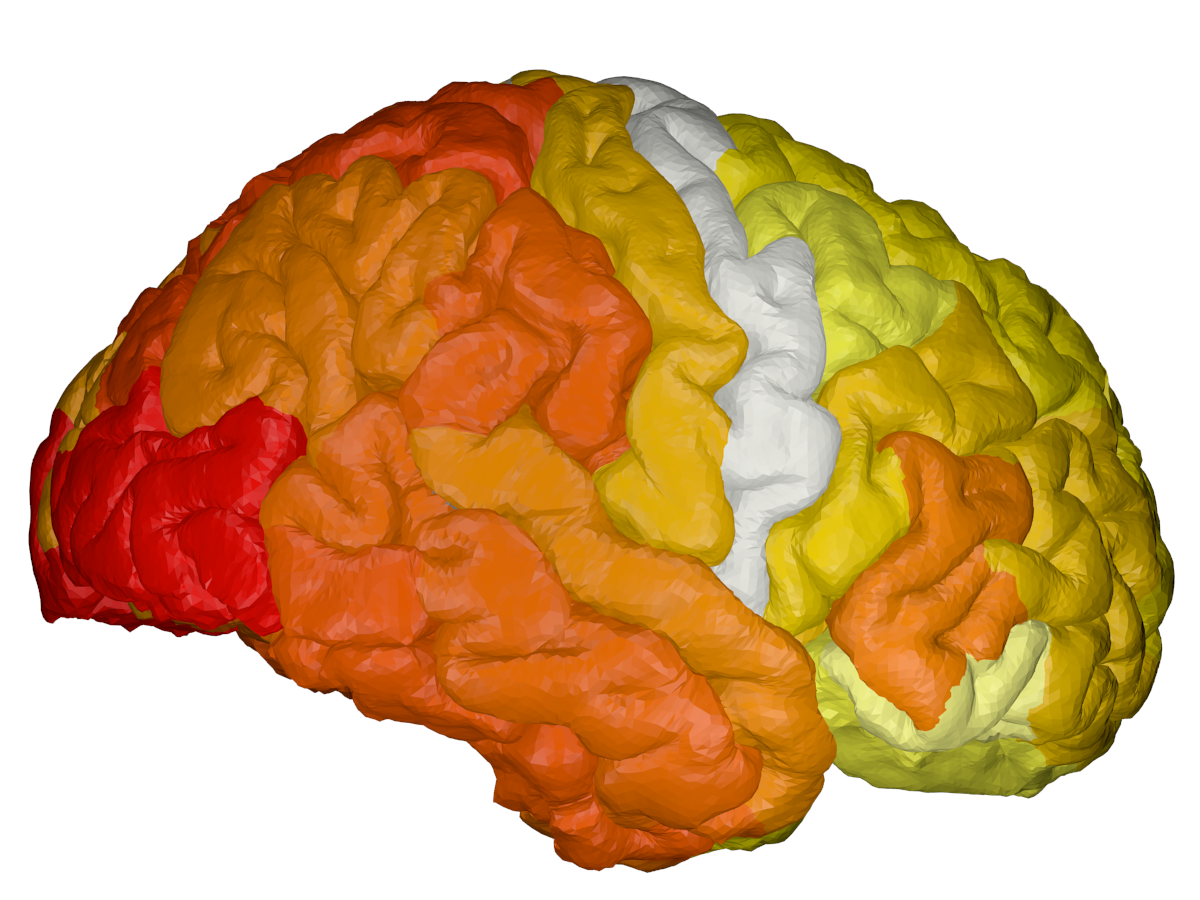
\includegraphics[height=2.3cm]{images/cortical-front_0.png}
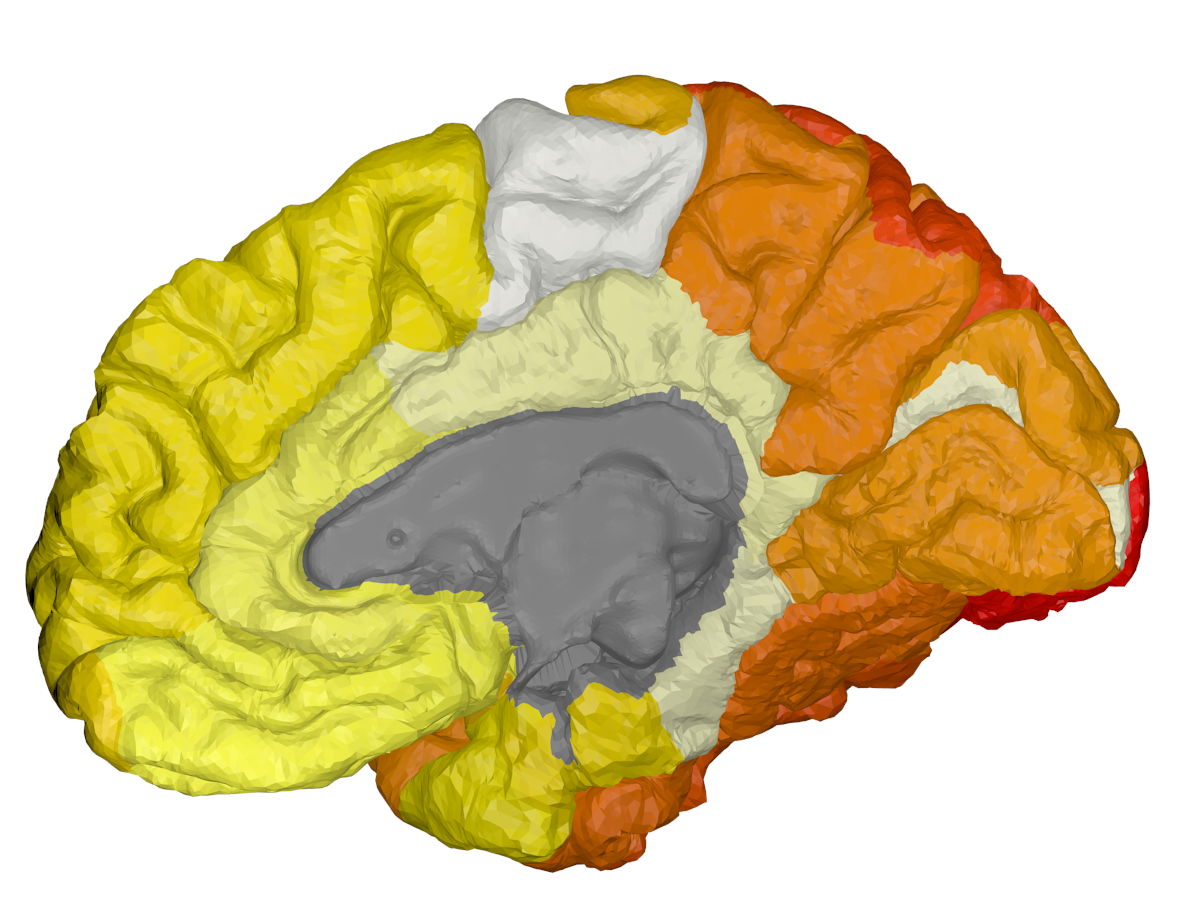
\includegraphics[height=2.3cm]{images/cortical-back_0.png}
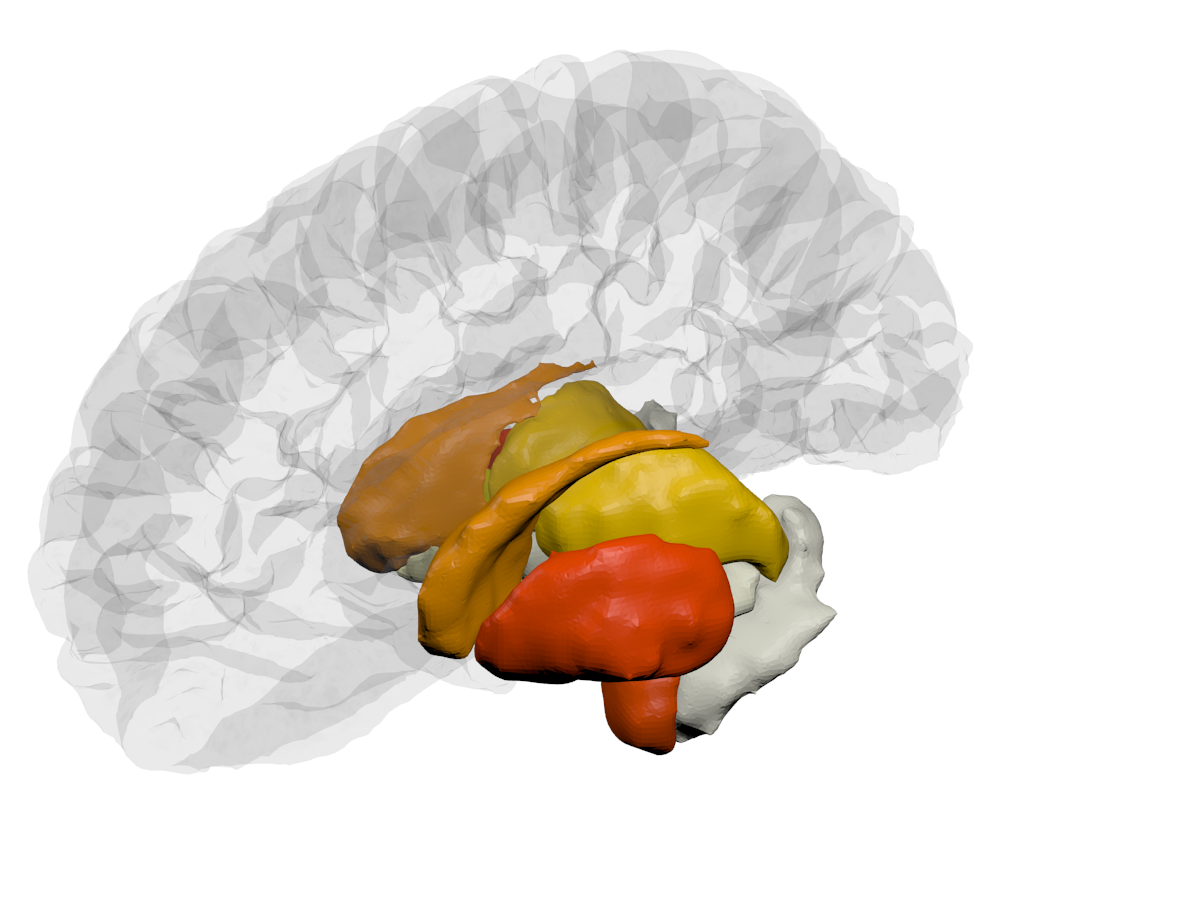
\includegraphics[height=2.3cm]{images/subcortical_0.png}
};
 \node (C2) at (C.north) {Brain 1};

    \node (D) at (-4,-8) {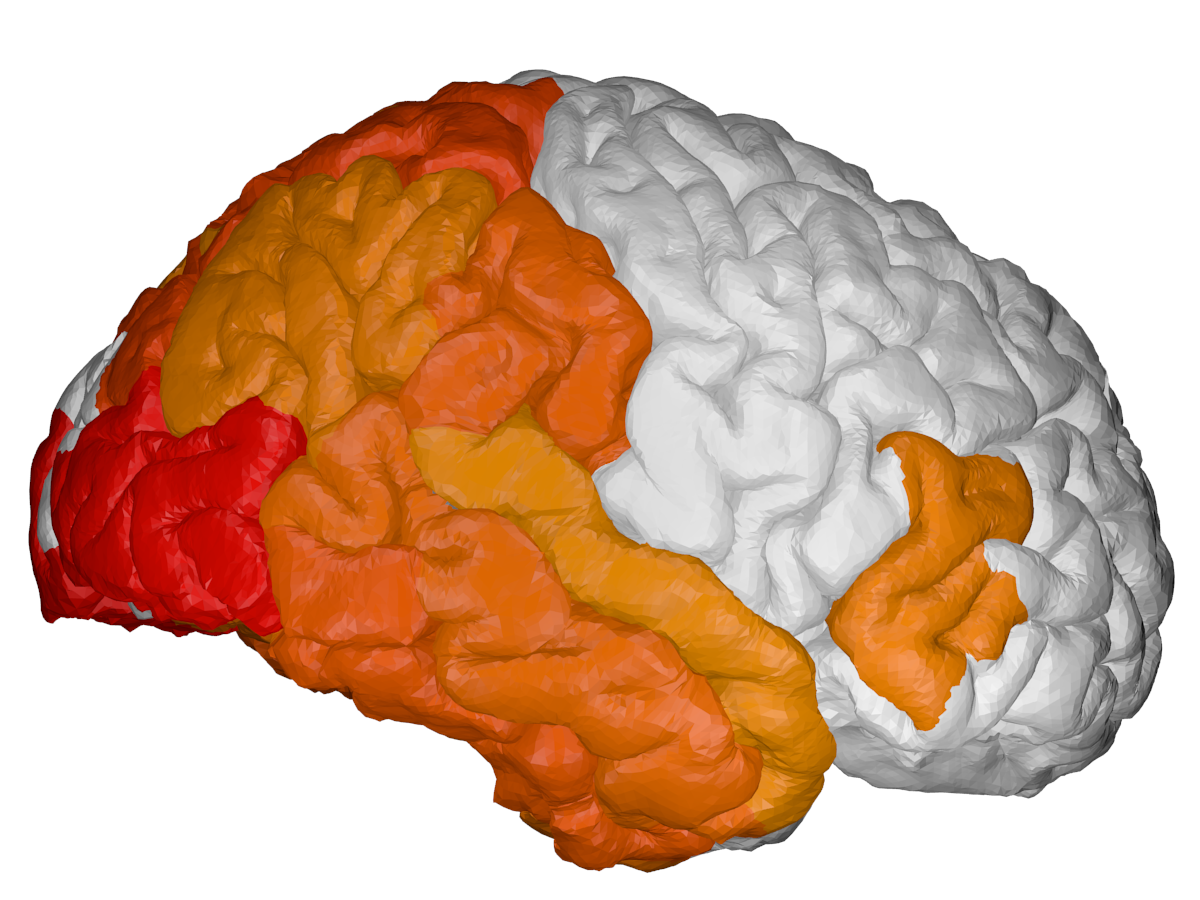
\includegraphics[height=2.3cm]{images/cortical-front_1.png}
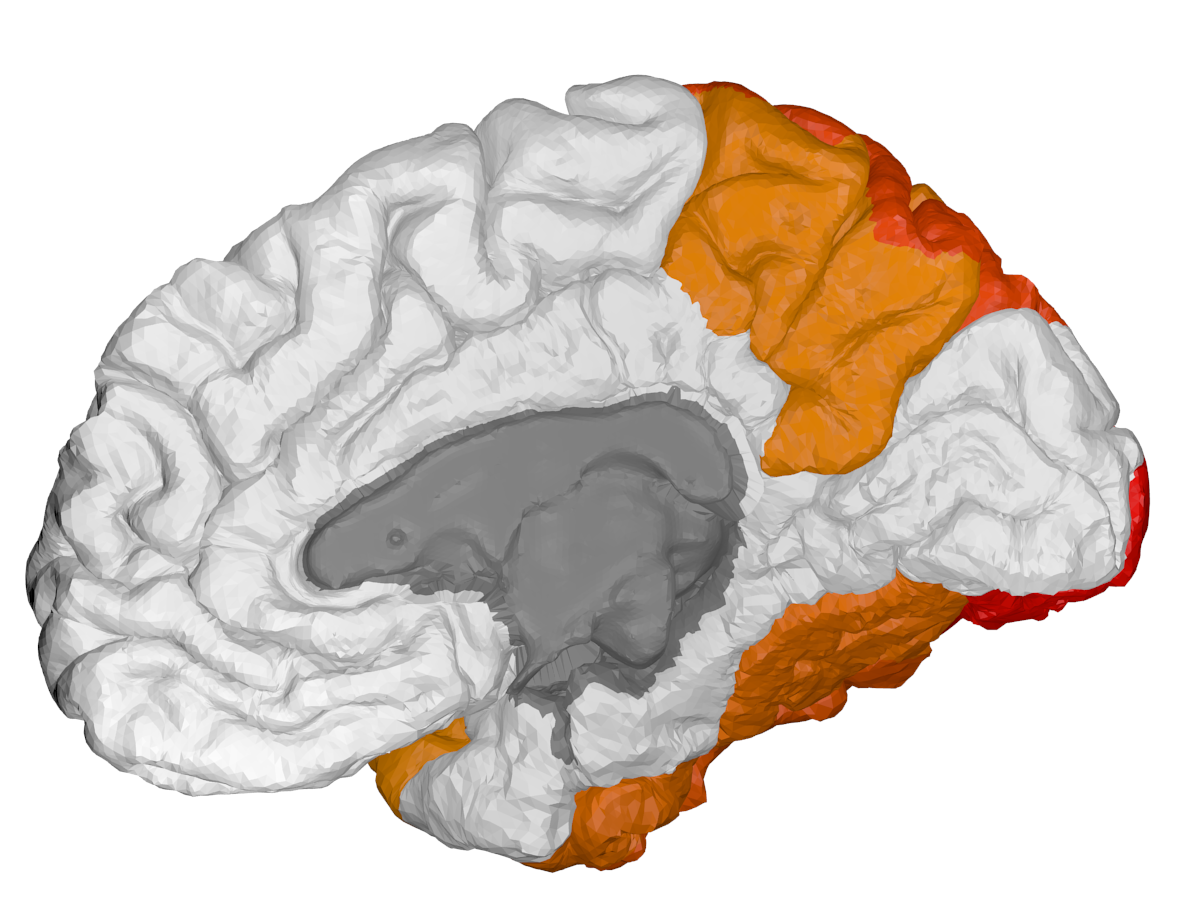
\includegraphics[height=2.3cm]{images/cortical-back_1.png}
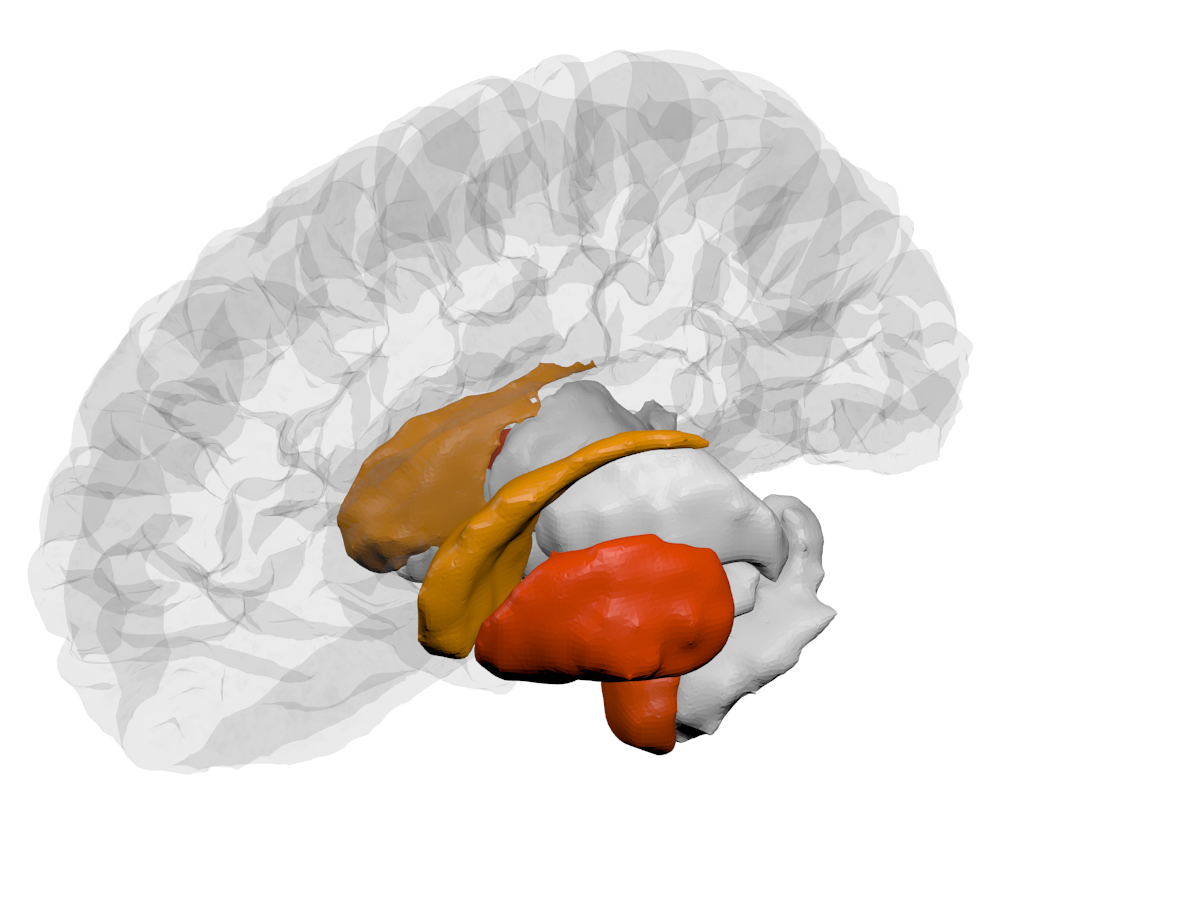
\includegraphics[height=2.3cm]{images/subcortical_1.png}};
 \node (D2) at (D.north) {Brain 2};

%     \draw[thick,->,shorten >= -2pt] (-2.7,4) -- (3,4) node[midway,above] {BrainPainter};
  \end{tikzpicture}
\captionof{figure}{Given a .csv file with region-of-interest (ROI) biomarkers and a user-defined color gradient, BrainPainter can automatically generate brain images with the cortical surface (left and middle) as well as with subcortical structures (right). The input .csv file can contain multiple rows, one for each set of output images. The color gradient is a list of RGB colours given by the user. Final colours are interpolated using the numbers from the input .csv file based on the color gradient -- e.g. if the hippocampus has an associated value of 1.2, it's final color in the output image will be an interpolation of colors 1 and 2 from the gradient.}
\label{fig:mainDiag}
\end{center}
% \vspace{-3em}
}


\begin{document}



\title{BrainPainter: A software for the visualisation of brain structures, biomarkers and associated pathological processes}
%
\titlerunning{BrainPainter: A software for the visualisation of brain structures, biomarkers and associated pathological processes}  % abbreviated title (for running head)
%                                     also used for the TOC unless
%                                     \toctitle is used
%


\author{***************}

\authorrunning{} % abbreviated author list (for running head)

\institute{***************}

% \institute{Centre for Medical Image Computing, University College London, UK
% \and 
% Queen Square MS Centre, UCL Institute of Neurology, UK
% \and 
% Dementia Research Centre, University College London, UK
% \and
% University of C\^{o}te d'Azur, Inria Sophia Antipolis, France
% % Laboratoire d'Analyse Num\'{e}rique, B\^{a}timent 425,\\
% % F-91405 Orsay Cedex, France}
% }


\maketitle              % typeset the title of the contribution


%\newcommand{\expFld}{../resfiles/tad-drcTiny_JMD}
\newcommand{\expFld}{.}


\begin{abstract}
We present BrainPainter, a software that automatically generates images of highlighted brain structures given a list of numbers corresponding to the output colours of each region. Compared to existing visualisation software (e.g. Freesurfer, SPM, 3D Slicer), our software has three key advantages: (1) it does not require the input data to be in a specialised format specific to the software, allowing it to be used in combination with any neuroimaging analsys tools, (2) it can visualise subcortical structures and (3) it can be used to generate movies showing dynamic processes, e.g. propagation of pathology on the brain, without requiring the user to write additional software code. We highlight two cases where BrainPainter was used in existing neuroimaging studies: visualisation of (1) the extent of atrophy through interpolation along a user-defined gradient of colours, as well as (2) progression of pathology in cortical and subcortical regions through snapshots. BrainPainter is available online \cite{brainPainter}. It is customisable, easy to use, and requires no installation, as it is distributed in a docker container.

% \keywords{Disease Progression Model, Transfer Learning, Manifold Learning, Alzheimer's Disease, Posterior Cortical Atrophy}
\end{abstract}


\section{Introduction}
\label{intro}



% diagram showing the aim: input numbers and output images

Visualisation of brain structure, function and pathology is crucial for understanding the mechanisms underlying certain neurodegenerative diseases and eases the interpretation of results in brain medical imaging. This is especially important in populations studies, where two or more populations are compared for any group differences in biomarkers derived from e.g. Magnetic Resonance Imaging, Positron Emmission Tomography (PET) or Computer Tomography (CT). However, for traumatic brain injury or rarer neurodegenerative diseases such as Parkinson's disease or Multiple Sclerosis, the visualisation of statistical results is sometimes not performed due to the inability to register images to a common template or lack of robust registration software, hence many studies such as \cite{coughlin2015neuroinflammation,mak2014subcortical,schoonheim2012subcortical,chard2002brain} only report differences between patients and controls in tables or as box plots. 

\frontFig

When alignment to a common population template is possible, e.g. in Alzheimer's disease, excellent 3D visualisation software exists  which allows interactive visualisation of population differences -- e.g. 3D Slicer \cite{pieper20043d}, Freesurfer \cite{fischl2012freesurfer} or SPM \cite{penny2011statistical}. However, such software have several inherent limitations. First, such software -- e.g. Freesurfer\footnote{We actually refer to Freeview, which is the visualisation software bundled with Freesurfer} -- generally requires inputs in their own data format, which is usually difficult and time-consuming to create without using their pipeline. Secondly, for highlighting complex patterns of pathology, authors need to show multiple slices from the same 3D image (sometimes from 4 \cite{seeley2009neurodegenerative} up to 8 slices \cite{migliaccio2015mapping}, which ends up taking too much space on the academic paper being publised. While Freesurfer solves this using a cortical surface-based representation that captures all the complexity of pathology patterns in a single image, it cannot visualise subcortical structures. Third, current visualisation software cannot be used to generate a movie showing a dynamic process, e.g. propagation of pathology within the human brain, without considerable effort modifying the software.

We present BrainPainter, a software for easy visualisation of structures, pathology and biomarkers in the brain. As opposed to previous visualisation software, the input data is a list of numbers in a .csv file representing colours to be assigned to each brain structure. Secondly, it can visualise patterns on both cortical and subcortical structures using a surface repreentation, removing the need to show multiple slices. Third, the images are generated automatically from pre-defined view-points, and can be used to create a movie showing e.g. the propagation of pathology, without the need to write any extra software code. BrainPainter is open source and available online \cite{brainPainter}.



%\FloatBarrier
\section{Design}
\label{design}

% diagram showing the Design. what kind of atlases can it take, type of colouring, blender integration


% how does BrianPainter work: takes input csv file, generates images. 
BrainPainter has a very simple workflow. Given an input csv file with biomarkers for each region, it produces high-quality visualisations of cortical and subcortical structures. For this, it uses Blender as a rendering engine, and loads 3D meshes of brain structures which are then coloured according to the input numbers.

% use of blender as rednering engine
BrianPainter uses open-source software Blender as the rendering engine. We chose Blender for two reasons. First, it is open-source, allowing us to distribute it already integrated with BrainPainter, thus requiring no further installation. Secondly, Blender is a powerful 3D graphics software, allowing one to set complex lightining conditions, handle transparency required for the glass-brain and also perform rendering from virtual cameras that can perform fly-overs around the brain. The software also supports a variety of object formats for the brain template, including the popular .obj mesh format.

% ATLASES: DK
The software is able to colour and visualise regions belonging to a pre-defined atlas. Currently, we support the Desikan-Killiany (DK) atlas \cite{desikan2006automated} and the Destrieux atlas \cite{destrieux2010automatic}. Moreover, if the input atlas does not match the DK or Destrieux atlas, the user is able to map the input regions to the DK or Destrieux atlas through a simple mapping in the config.py \footnote{URL anonymised for blind review} file.  % \footnote{\url{https://github.com/mrazvan22/brain-coloring/blob/master/config.py}}

% customisation

BrainPainter can be easily customised in several ways through the config.py settings file. First of all, the colours assigned to each region can be changed. Moreover, we support interpolating through multiple colors on a gradient, for example from white $\rightarrow$ yellow $\rightarrow$ orange $\rightarrow$ red, as in the example from Fig. \ref{fig:mainDiag}. In this case, the input numbers need to be in the range [0,3], where a value of 1.3 would interpolate between colour 1 (yellow) and color 2 (orange). The resolution and the background colour can also be changed. More complex settings such as the viewing angle can be customised from \verb|blendHelper.py:setCamera()|, while luminosity settings can also be changed from \verb|blendHelper.py:setLamp()|. In the future, we plan to integrate the most important such settings into config.py. 

% Docker containers
In order to remove the need to install Blender and other dependencies, BrainPainter is distributed into a docker container with pre-installed Blender and the python dependencies. 


\begin{figure}
\centering
 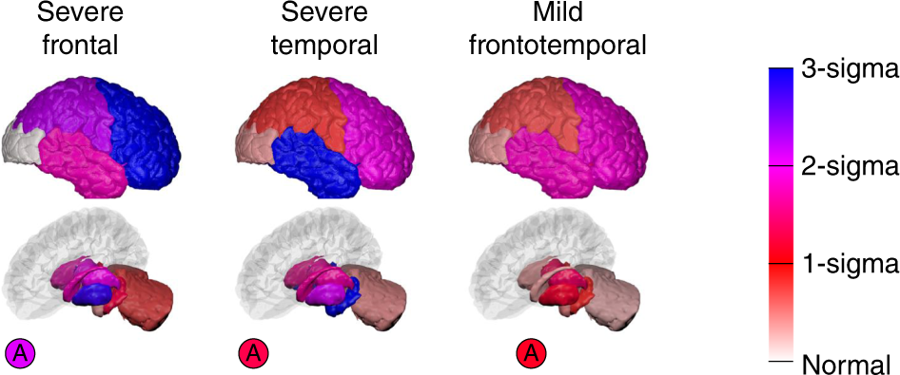
\includegraphics[width=0.8\textwidth]{images/young_3brains.png}
 \caption{Demonstration of BrainPainter for showing extent of pathology on a vertical bar, where colours towards blue show increased severity. Source: \cite{young2018uncovering}.}
 \label{fig:youngExtent}
\end{figure}

\begin{figure*}[htp]
\centering
 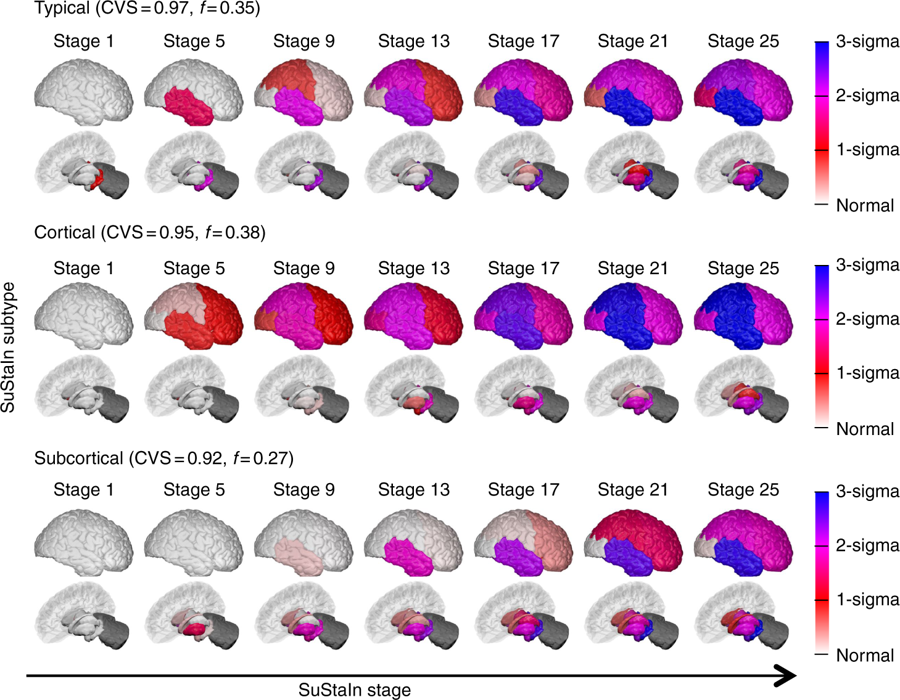
\includegraphics[width=1\textwidth, trim=20 0 0 220, clip]{images/young_progression.png}
 \caption{Demonstration of our software for showing the temporal progression of pathology, as a sequence of snapshot at different stages. Images used by \cite{young2018uncovering}.}
  \label{fig:youngProg}
\end{figure*}

\section{Use case 1: Extent of pathology}
\label{extent}

BrainPainter can be used to show the severity of pathology within the human brain. This can be highlighted with different colours that can be customised by the user. An example of such an application if shown in Fig. \ref{fig:youngExtent}, where regions with no pathology are coloured in white and very severe regions are coloured in blue. A gradient such as the one on the right can be used to map the colours to some problem-specific labels.




\section{Use case 2: Temporal progression of pathology}
\label{progression}

Our software can be used to show dynamic processes in the human brain, such as the temporal progression of pathology, as a series of snapshots. For this, one simply needs to provide multiple rows in the input csv, one for each snapshot. Two demonstrations are shown in Fig. \ref{fig:youngProg} and Fig. \ref{fig:peter}.



\begin{figure}[htp]
\centering
% \subfigure{Stage 0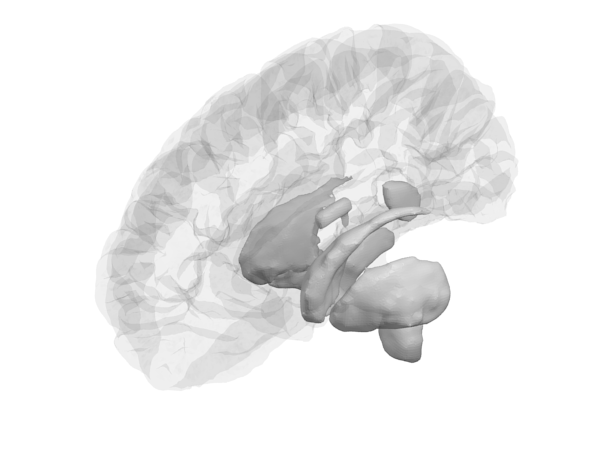
\includegraphics[width=0.2\textwidth]{images/ebmhd_pngs/subcortical_stage0.png}}
\subfloat[Stage 0]{
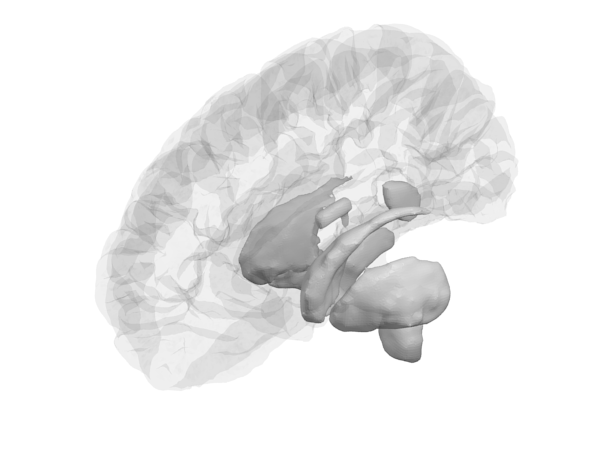
\includegraphics[width=0.2\textwidth,trim=70 0 70 0, clip]{images/ebmhd_pngs/subcortical_stage0.png}}
\subfloat[Stage 3]{
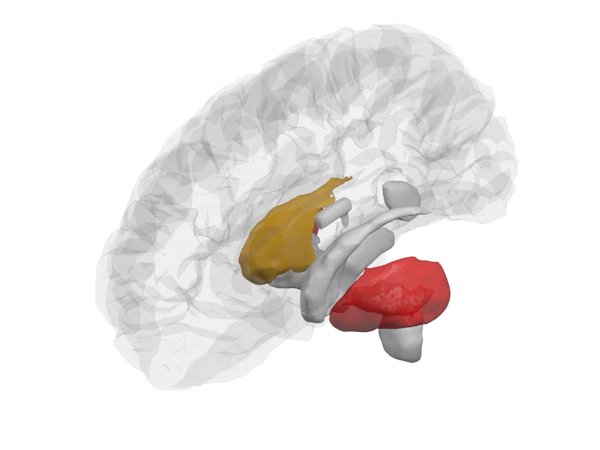
\includegraphics[width=0.2\textwidth,trim=70 0 70 0, clip]{images/ebmhd_pngs/subcortical_stage3.png}}

\subfloat[Stage 7]{
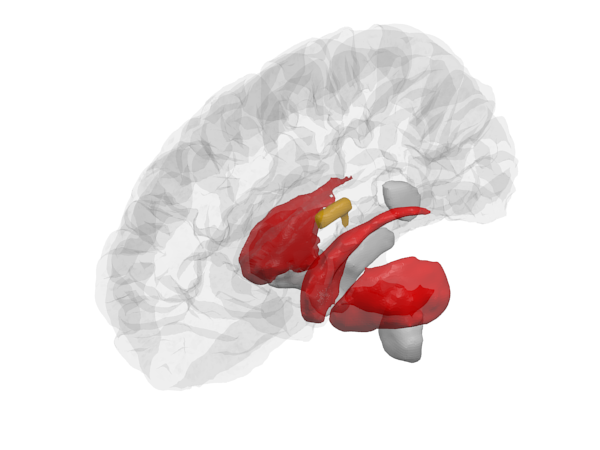
\includegraphics[width=0.2\textwidth,trim=70 0 70 0, clip]{images/ebmhd_pngs/subcortical_stage7.png}}
\subfloat[Stage 10]{
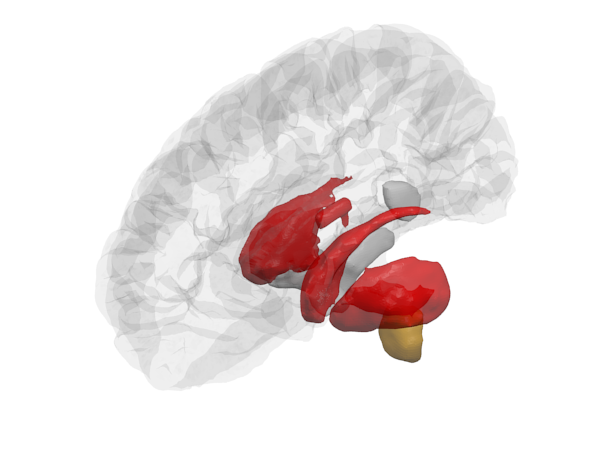
\includegraphics[width=0.2\textwidth,trim=70 0 70 0, clip]{images/ebmhd_pngs/subcortical_stage10.png}}
 \caption{Progression of pathology in subcortical regions within a glass brain, using images generated with our method. Images used by \cite{wijeratne2018image}.}
   \label{fig:peter}
\end{figure}

\section{Limitations}

Our software has several limitations that can be addressed in future versions. First of all, we currently only support the DK and Destrieux atlases as these were the only 3D meshes available online\footnote{https://brainder.org/research/brain-for-blender/}. Secondly, it can currently only highlight entire regions-of-interest from such an atlas. However, showing fine-grained voxelwise/vertexwise patterns of colouring requires a specialised input format, which the users will need to convert their data to -- for usability, we decided to only enable coloring based on atlases, although future versions can include the ability to highlight fine-grained patterns. Yet another limitation of BrainPainter is that it cannot visualise more complex structures such as white-matter tracts, although we are happy to add such functionality if there is interest for it within the neuroimaging community.


\section{Conclusion}

We presented BrainPainter, an open-source software that can be used to visualise structures, biomarkers and pathologies in the human brain. BrainPainter is easy to use, requires no installation, and accepts input data in a .csv format there each column represents biomarkers in a specific brain region. 

The visualisations generated by BrainPainter can be used to significantly enhance the interpretation of neuroimaging research. The generated images can be easily embedded by researchers into their scientific articles. Moreover, it can also easily generate movies showing dynamic processes, e.g. propagation of pathology, within the human brain. 



\FloatBarrier
\section{Acknowledgements}


RVM was supported by the EPSRC Centre For Doctoral Training in Medical Imaging with grant EP/L016478/1, as well as NIH grants NIBIB NAC P41EB015902 and NINDS R01NS086905. DCA was supported by EuroPOND, which is an EU Horizon 2020 project, and by EPSRC grants J020990, M006093 and M020533. PG was supported by NIH grants NIBIB NAC P41EB015902 and NINDS R01NS086905. 

% \section{References}

\bibliographystyle{splncs}
\bibliography{bibliography}

% \bibliographystyle{unsrtnat}
% \begin{thebibliography}{5}
% 
% \bibitem{jack2010hypothetical}
% Jack, C.R., Knopman, D.S., Jagust, W.J., Shaw, L.M., Aisen, P.S., Weiner, M.W., Petersen, R.C. and Trojanowski, J.Q., 2010. Hypothetical model of dynamic biomarkers of the Alzheimer's pathological cascade. The Lancet Neurology, 9(1), pp.119-128.
% 
% \bibitem{bateman2012clinical}
% Bateman, R.J., Xiong, C., Benzinger, T.L., Fagan, A.M., Goate, A., Fox, N.C., Marcus, D.S., Cairns, N.J., Xie, X., Blazey, T.M. and Holtzman, D.M., 2012. Clinical and biomarker changes in dominantly inherited Alzheimer's disease. New England Journal of Medicine, 367(9), pp.795-804.
% 
% \bibitem{richberg2015multi}
% Schmidt-Richberg, A., Guerrero, R., Ledig, C., Molina-Abril, H., Frangi, A.F., Rueckert, D. and Alzheimers Disease Neuroimaging Initiative, 2015, June. Multi-stage Biomarker Models for Progression Estimation in Alzheimer’s Disease. In International Conference on Information Processing in Medical Imaging (pp. 387-398). Springer International Publishing.
% 
% \bibitem{fonteijn2012event}
% Fonteijn, H.M., Modat, M., Clarkson, M.J., Barnes, J., Lehmann, M., Hobbs, N.Z., Scahill, R.I., Tabrizi, S.J., Ourselin, S., Fox, N.C. and Alexander, D.C., 2012. An event-based model for disease progression and its application in familial Alzheimer's disease and Huntington's disease. NeuroImage, 60(3), pp.1880-1889.
% 
% \bibitem {jedynak2012}
% Jedynak, B.M., Lang, A., Liu, B., Katz, E., Zhang, Y., Wyman, B.T., Raunig, D., Jedynak, C.P., Caffo, B., Prince, J.L. and Alzheimer's Disease Neuroimaging Initiative, 2012. A computational neurodegenerative disease progression score: method and results with the Alzheimer's Disease Neuroimaging Initiative cohort. Neuroimage, 63(3), pp.1478-1486.
% 
% \bibitem{donohue2014estimating}
% Donohue, M.C., Jacqmin-Gadda, H., Le Goff, M., Thomas, R.G., Raman, R., Gamst, A.C., Beckett, L.A., Jack, C.R., Weiner, M.W., Dartigues, J.F. and Aisen, P.S., 2014. Estimating long-term multivariate progression from short-term data. Alzheimer's \& Dementia, 10(5), pp.S400-S410.
% 
% \bibitem{schiratti2015mixed}
% Schiratti, J.B., Allassonniere, S., Routier, A., Colliot, O., Durrleman, S. and Alzheimers Disease Neuroimaging Initiative, 2015, June. A mixed-effects model with time reparametrization for longitudinal univariate manifold-valued data. In International Conference on Information Processing in Medical Imaging (pp. 564-575). Springer International Publishing.
% 
% \bibitem{bilgel2016multivariate}
% Bilgel, M., Prince, J.L., Wong, D.F., Resnick, S.M. and Jedynak, B.M., 2016. A multivariate nonlinear mixed effects model for longitudinal image analysis: Application to amyloid imaging. NeuroImage, 134, pp.658-670.
% 
% \bibitem{seeley2009neurodegenerative}
% Seeley, W.W., Crawford, R.K., Zhou, J., Miller, B.L. and Greicius, M.D., 2009. Neurodegenerative diseases target large-scale human brain networks. Neuron, 62(1), pp.42-52.
% 
% % \bibitem{bishop2006}
% % Bishop, C.M., 2006. Pattern recognition. Machine Learning, 128.
% 
% \bibitem{reuter2012longitudinal}
% Reuter, M., Schmansky, N.J., Rosas, H.D. and Fischl, B., 2012. Within-subject template estimation for unbiased longitudinal image analysis. Neuroimage, 61(4), pp.1402-1418.
% 
% % \bibitem{reuter2010inverse}
% % Reuter, M., Rosas, H.D. and Fischl, B., 2010. Highly accurate inverse consistent registration: a robust approach. Neuroimage, 53(4), pp.1181-1196.
% 
% \bibitem{dickerson2009cortical}
% Dickerson, B.C., Bakkour, A., Salat, D.H., Feczko, E., Pacheco, J., Greve, D.N., Grodstein, F., Wright, C.I., Blacker, D., Rosas, H.D. and Sperling, R.A., 2009. The cortical signature of Alzheimer's disease: regionally specific cortical thinning relates to symptom severity in very mild to mild AD dementia and is detectable in asymptomatic amyloid-positive individuals. Cerebral cortex, 19(3), pp.497-510.
% 
% % \bibitem{thompson2001cortical}
% % Thompson, P.M., Mega, M.S., Woods, R.P., Zoumalan, C.I., Lindshield, C.J., Blanton, R.E., Moussai, J., Holmes, C.J., Cummings, J.L. and Toga, A.W., 2001. Cortical change in Alzheimer's disease detected with a disease-specific population-based brain atlas. Cerebral Cortex, 11(1), pp.1-16.
% 
% \bibitem{crutch2012posterior}
% Crutch, S.J., Lehmann, M., Schott, J.M., Rabinovici, G.D., Rossor, M.N. and Fox, N.C., 2012. Posterior cortical atrophy. The Lancet Neurology, 11(2), pp.170-178.
% 
% \bibitem{young2015multiple}
% Young, A.L., Oxtoby, N.P., Huang, J., Marinescu, R.V., Daga, P., Cash, D.M., Fox, N.C., Ourselin, S., Schott, J.M., Alexander, D.C. and Alzheimers Disease Neuroimaging Initiative, 2015, June. Multiple Orderings of Events in Disease Progression. In International Conference on Information Processing in Medical Imaging (pp. 711-722). Springer International Publishing.
% 
% \end{thebibliography}




\end{document}




\endinput


%%
%% End of file `elsarticle-template-harv.tex'.
